\documentclass{standalone}
\usepackage{tikz}
\usetikzlibrary{patterns, positioning}


\begin{document}
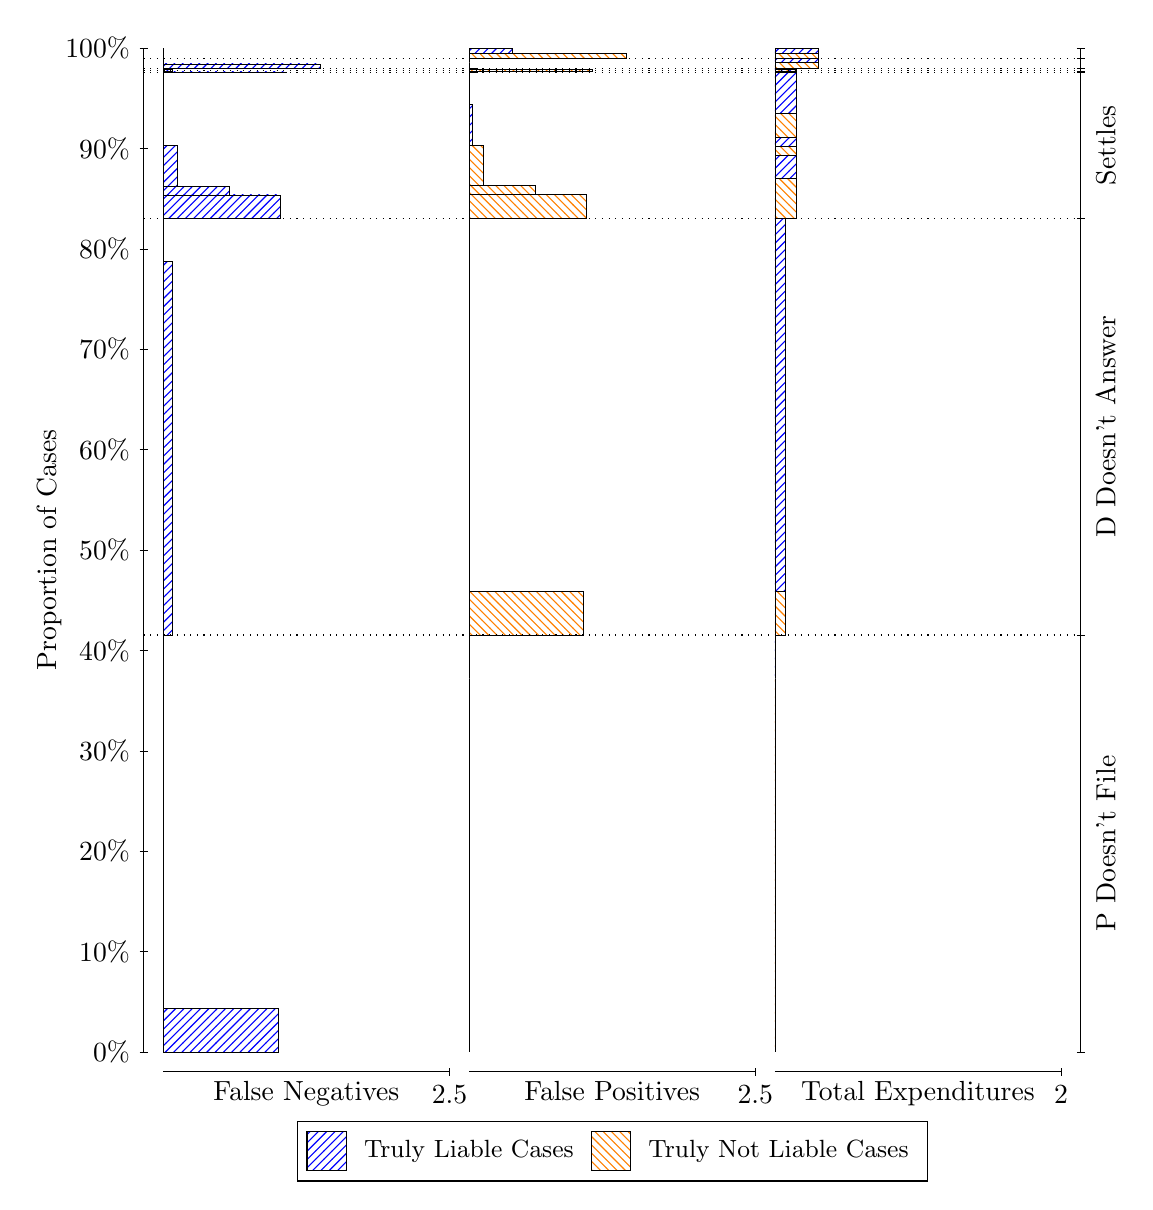
\begin{tikzpicture}
\draw[black, very thin] (1.5,1.75) -- (1.5,14.5);
\node[rotate=90, text=black, anchor=center] at (0.3, 8.125) {Proportion of Cases};
\draw[black, very thin] (1.45,1.75) -- (1.55,1.75);
\node[text=black, anchor=east] at (1.45, 1.75) {0\%};
\draw[black, very thin] (1.45,3.025) -- (1.55,3.025);
\node[text=black, anchor=east] at (1.45, 3.025) {10\%};
\draw[black, very thin] (1.45,4.3) -- (1.55,4.3);
\node[text=black, anchor=east] at (1.45, 4.3) {20\%};
\draw[black, very thin] (1.45,5.575) -- (1.55,5.575);
\node[text=black, anchor=east] at (1.45, 5.575) {30\%};
\draw[black, very thin] (1.45,6.85) -- (1.55,6.85);
\node[text=black, anchor=east] at (1.45, 6.85) {40\%};
\draw[black, very thin] (1.45,8.125) -- (1.55,8.125);
\node[text=black, anchor=east] at (1.45, 8.125) {50\%};
\draw[black, very thin] (1.45,9.4) -- (1.55,9.4);
\node[text=black, anchor=east] at (1.45, 9.4) {60\%};
\draw[black, very thin] (1.45,10.675) -- (1.55,10.675);
\node[text=black, anchor=east] at (1.45, 10.675) {70\%};
\draw[black, very thin] (1.45,11.95) -- (1.55,11.95);
\node[text=black, anchor=east] at (1.45, 11.95) {80\%};
\draw[black, very thin] (1.45,13.225) -- (1.55,13.225);
\node[text=black, anchor=east] at (1.45, 13.225) {90\%};
\draw[black, very thin] (1.45,14.5) -- (1.55,14.5);
\node[text=black, anchor=east] at (1.45, 14.5) {100\%};

\draw[black, very thin] (13.4,1.75) -- (13.4,14.5);
\draw[black, very thin] (13.35,1.75) -- (13.45,1.75);
\node[anchor=west] at (13.35, 1.75) {};
\draw[black, very thin] (13.35,7.0451) -- (13.45,7.0451);
\node[anchor=west] at (13.35, 7.0451) {};
\draw[black, very thin] (13.35,12.34) -- (13.45,12.34);
\node[anchor=west] at (13.35, 12.34) {};
\draw[black, very thin] (13.35,14.191) -- (13.45,14.191);
\node[anchor=west] at (13.35, 14.191) {};
\draw[black, very thin] (13.35,14.211) -- (13.45,14.211);
\node[anchor=west] at (13.35, 14.211) {};
\draw[black, very thin] (13.35,14.242) -- (13.45,14.242);
\node[anchor=west] at (13.35, 14.242) {};
\draw[black, very thin] (13.35,14.372) -- (13.45,14.372);
\node[anchor=west] at (13.35, 14.372) {};
\draw[black, very thin] (13.35,14.5) -- (13.45,14.5);
\node[anchor=west] at (13.35, 14.5) {};

\draw[black, very thin, pattern color=blue, pattern=north east lines] (1.75,1.75) rectangle (3.2033,2.303);
\draw[black, very thin, pattern color=orange, pattern=north west lines] (1.75,2.303) rectangle (1.75,7.0451);
\draw[black, very thin, pattern color=blue, pattern=north east lines] (1.75,7.0451) rectangle (1.859,11.787);
\draw[black, very thin, pattern color=orange, pattern=north west lines] (1.75,11.787) rectangle (1.75,12.34);
\draw[black, very thin, pattern color=blue, pattern=north east lines] (1.75,12.34) rectangle (3.2397,12.634);
\draw[black, very thin, pattern color=blue, pattern=north east lines] (1.75,12.634) rectangle (2.5857,12.746);
\draw[black, very thin, pattern color=blue, pattern=north east lines] (1.75,12.746) rectangle (1.9317,13.268);
\draw[black, very thin, pattern color=orange, pattern=north west lines] (1.75,13.268) rectangle (1.75,14.191);
\draw[black, very thin, pattern color=blue, pattern=north east lines] (1.75,14.191) rectangle (3.3123,14.198);
\draw[black, very thin, pattern color=orange, pattern=north west lines] (1.75,14.198) rectangle (1.75,14.211);
\draw[black, very thin, pattern color=blue, pattern=north east lines] (1.75,14.211) rectangle (1.859,14.227);
\draw[black, very thin, pattern color=orange, pattern=north west lines] (1.75,14.227) rectangle (1.75,14.242);
\draw[black, very thin, pattern color=blue, pattern=north east lines] (1.75,14.242) rectangle (3.7483,14.298);
\draw[black, very thin, pattern color=orange, pattern=north west lines] (1.75,14.298) rectangle (1.75,14.372);
\draw[black, very thin, pattern color=orange, pattern=north west lines] (1.75,14.372) rectangle (1.75,14.427);
\draw[black, very thin, pattern color=blue, pattern=north east lines] (1.75,14.427) rectangle (1.75,14.5);
\draw[black, very thin, pattern color=orange, pattern=north west lines] (5.6333,1.75) rectangle (5.6333,6.492);
\draw[black, very thin, pattern color=blue, pattern=north east lines] (5.6333,6.492) rectangle (5.6333,7.0451);
\draw[black, very thin, pattern color=orange, pattern=north west lines] (5.6333,7.0451) rectangle (7.0867,7.5979);
\draw[black, very thin, pattern color=blue, pattern=north east lines] (5.6333,7.5979) rectangle (5.6333,12.34);
\draw[black, very thin, pattern color=orange, pattern=north west lines] (5.6333,12.34) rectangle (7.123,12.645);
\draw[black, very thin, pattern color=orange, pattern=north west lines] (5.6333,12.645) rectangle (6.469,12.757);
\draw[black, very thin, pattern color=orange, pattern=north west lines] (5.6333,12.757) rectangle (5.815,13.263);
\draw[black, very thin, pattern color=blue, pattern=north east lines] (5.6333,13.263) rectangle (5.6697,13.784);
\draw[black, very thin, pattern color=blue, pattern=north east lines] (5.6333,13.784) rectangle (5.6333,14.191);
\draw[black, very thin, pattern color=orange, pattern=north west lines] (5.6333,14.191) rectangle (5.7423,14.204);
\draw[black, very thin, pattern color=blue, pattern=north east lines] (5.6333,14.204) rectangle (5.6333,14.211);
\draw[black, very thin, pattern color=orange, pattern=north west lines] (5.6333,14.211) rectangle (7.1957,14.227);
\draw[black, very thin, pattern color=blue, pattern=north east lines] (5.6333,14.227) rectangle (5.7423,14.242);
\draw[black, very thin, pattern color=orange, pattern=north west lines] (5.6333,14.242) rectangle (5.6333,14.317);
\draw[black, very thin, pattern color=blue, pattern=north east lines] (5.6333,14.317) rectangle (5.6333,14.372);
\draw[black, very thin, pattern color=orange, pattern=north west lines] (5.6333,14.372) rectangle (7.6317,14.427);
\draw[black, very thin, pattern color=blue, pattern=north east lines] (5.6333,14.427) rectangle (6.1783,14.5);
\draw[black, very thin, pattern color=orange, pattern=north west lines] (9.5167,1.75) rectangle (9.5167,6.492);
\draw[black, very thin, pattern color=blue, pattern=north east lines] (9.5167,6.492) rectangle (9.5167,7.0451);
\draw[black, very thin, pattern color=orange, pattern=north west lines] (9.5167,7.0451) rectangle (9.6529,7.5979);
\draw[black, very thin, pattern color=blue, pattern=north east lines] (9.5167,7.5979) rectangle (9.6529,12.34);
\draw[black, very thin, pattern color=orange, pattern=north west lines] (9.5167,12.34) rectangle (9.7892,12.845);
\draw[black, very thin, pattern color=blue, pattern=north east lines] (9.5167,12.845) rectangle (9.7892,13.14);
\draw[black, very thin, pattern color=orange, pattern=north west lines] (9.5167,13.14) rectangle (9.7892,13.252);
\draw[black, very thin, pattern color=blue, pattern=north east lines] (9.5167,13.252) rectangle (9.7892,13.364);
\draw[black, very thin, pattern color=orange, pattern=north west lines] (9.5167,13.364) rectangle (9.7892,13.669);
\draw[black, very thin, pattern color=blue, pattern=north east lines] (9.5167,13.669) rectangle (9.7892,14.191);
\draw[black, very thin, pattern color=orange, pattern=north west lines] (9.5167,14.191) rectangle (9.7892,14.204);
\draw[black, very thin, pattern color=blue, pattern=north east lines] (9.5167,14.204) rectangle (9.7892,14.211);
\draw[black, very thin, pattern color=orange, pattern=north west lines] (9.5167,14.211) rectangle (9.7892,14.227);
\draw[black, very thin, pattern color=blue, pattern=north east lines] (9.5167,14.227) rectangle (9.7892,14.242);
\draw[black, very thin, pattern color=orange, pattern=north west lines] (9.5167,14.242) rectangle (10.062,14.317);
\draw[black, very thin, pattern color=blue, pattern=north east lines] (9.5167,14.317) rectangle (10.062,14.372);
\draw[black, very thin, pattern color=orange, pattern=north west lines] (9.5167,14.372) rectangle (10.062,14.427);
\draw[black, very thin, pattern color=blue, pattern=north east lines] (9.5167,14.427) rectangle (10.062,14.5);
\draw[black, dotted] (1.5,7.0451) -- (13.4,7.0451);
\draw[black, dotted] (1.5,12.34) -- (13.4,12.34);
\draw[black, dotted] (1.5,14.191) -- (13.4,14.191);
\draw[black, dotted] (1.5,14.211) -- (13.4,14.211);
\draw[black, dotted] (1.5,14.242) -- (13.4,14.242);
\draw[black, dotted] (1.5,14.372) -- (13.4,14.372);
\draw[black, very thin] (1.75,1.5) -- (5.3833,1.5);
\node[text=black, anchor=north] at (3.5667, 1.5) {False Negatives};
\draw[black, very thin] (5.3833,1.45) -- (5.3833,1.55);
\node[text=black, anchor=north] at (5.3833, 1.45) {2.5};

\draw[black, very thin] (5.6333,1.5) -- (9.2667,1.5);
\node[text=black, anchor=north] at (7.45, 1.5) {False Positives};
\draw[black, very thin] (9.2667,1.45) -- (9.2667,1.55);
\node[text=black, anchor=north] at (9.2667, 1.45) {2.5};

\draw[black, very thin] (9.5167,1.5) -- (13.15,1.5);
\node[text=black, anchor=north] at (11.333, 1.5) {Total Expenditures};
\draw[black, very thin] (13.15,1.45) -- (13.15,1.55);
\node[text=black, anchor=north] at (13.15, 1.45) {2};

\node[text=black, centered, rotate=90] at (13.72, 4.3975) {P Doesn't File};
\node[text=black, centered, rotate=90] at (13.72, 9.6924) {D Doesn't Answer};
\node[text=black, centered, rotate=90] at (13.72, 13.265) {Settles};





\draw (7.449999999999999,1.5) node[draw=none] (baseCoordinate) {};
\begin{scope}[align=center]
        \matrix[scale=0.5, draw=black, below=0.5cm of baseCoordinate, nodes={draw}, column sep=0.1cm]{
            \node[rectangle, draw, minimum width=0.5cm, minimum height=0.5cm, pattern color=blue, pattern=north east lines] {}; &
            \node[draw=none, font=\small, text=black] (B) {Truly Liable Cases}; &
            \node[rectangle, draw, minimum width=0.5cm, minimum height=0.5cm, pattern color=orange, pattern=north west lines] {}; &
            \node[draw=none, font=\small, text=black] (B) {Truly Not Liable Cases}; \\
            };
\end{scope}

\end{tikzpicture}
\end{document}